\documentclass[a4paper,12pt]{article}
\usepackage[utf8]{inputenc}
\usepackage{babel}
\usepackage{amsmath}
\usepackage{amssymb}
\usepackage{amsthm}
\usepackage{geometry}
\usepackage{graphicx}
\usepackage[hidelinks]{hyperref}
\usepackage{listings}
\usepackage{xcolor}
\usepackage{enumitem}
\usepackage{microtype}

\geometry{margin=2.5cm}

\microtypesetup{protrusion=true,expansion=true,stretch=30,shrink=30}

% Aggressive Overfull-Prävention
\emergencystretch=2em
\sloppy
\hbadness=10000
\vbadness=10000

\theoremstyle{definition}
\newtheorem{definition}{Definition}[section]
\newtheorem{beispiel}{Beispiel}[section]
\newtheorem{satz}{Satz}[section]
\newtheorem{lemma}{Lemma}[section]
\newtheorem{bemerkung}{Bemerkung}[section]
\newtheorem{korollar}{Korollar}[section]

% Deutsche Übersetzungen
\renewcommand{\proofname}{Beweis}
\renewcommand{\contentsname}{Inhaltsverzeichnis}
\renewcommand{\abstractname}{Zusammenfassung}
\renewcommand{\refname}{Literaturverzeichnis}
\renewcommand{\tablename}{Tabelle}
\renewcommand{\figurename}{Abbildung}

\setlist[itemize,1]{label=--}

% ---------- Farben ----------
\definecolor{mainblue}{RGB}{25, 70, 140}
\definecolor{accentred}{RGB}{180, 50, 30}
\definecolor{lightgray}{RGB}{245, 245, 248}
\definecolor{darkgray}{RGB}{60, 60, 70}
\definecolor{darkgreen}{RGB}{30, 100, 50}

\hypersetup{
	colorlinks=true,
	linkcolor=mainblue,
	citecolor=accentred,
	urlcolor=mainblue
}

%  Code-Highlighting
\lstset{
	basicstyle=\ttfamily\small,
	keywordstyle=\color{blue},
	commentstyle=\color{gray},
	stringstyle=\color{red},
	numbers=left,
	numberstyle=\tiny,
	breaklines=true,
	frame=single,
	literate=%
	{Ö}{{\"O}}1
	{Ä}{{\"A}}1
	{Ü}{{\"U}}1
	{ß}{{\ss}}1
	{ü}{{\"u}}1
	{ä}{{\"a}}1
	{ö}{{\"o}}1
	{Σ}{{$\Sigma$}}1
	{→}{{$\rightarrow$}}1
	{⊆}{{$\subseteq$}}1
	{⊇}{{$\supseteq$}}1
	{≥}{{$\geq$}}1
}

\title{Polynomielle Reduktion von Parameterisierten Problemen\\auf das Subgraph Isomorphismus-Problem}
\author{Stephan Epp}
\date{3. Juli 2026}

\begin{document}
	
\maketitle

\tableofcontents
\newpage

\section{Einführung}

Die Theorie der parameterisierten Komplexität bietet einen verfeinerten Blick auf die Lösbarkeit von algorithmischen Problemen. Während die klassische Komplexitätstheorie die Laufzeit nur als Funktion der Eingabegröße analysiert, berücksichtigt die parameterisierte Komplexität zusätzliche strukturelle Parameter der Eingabeinstanz. Ein Problem ist \emph{fixed-parameter tractable} (FPT), wenn es in Laufzeit $f(k) \cdot n^c$ lösbar ist, wobei $k$ ein Parameter, $n$ die Eingabegröße und $f$ eine beliebige berechenbare Funktion ist.

Die zentrale These dieser Arbeit ist, dass drei klassische NP-vollständige Probleme der parameterisierten Algorithmik – Min-Ones-2-SAT, Multicolored Clique und Set-Cover – durch polynomielle Reduktion auf das Subgraph Isomorphismus-Problem lösbar sind. Der Subgraph Algorithmus (siehe \cite{subgraph2026}), der das Subgraph Isomorphismus-Problem in $O(n^3)$ Zeit löst, bildet damit ein universelles Löungswerkzeug für diese und verwandte parameterisierte Probleme.

\subsection{Motivation}

Die praktische Relevanz dieser Reduktion liegt in mehreren Punkten:

\begin{itemize}
	\item \textbf{Universelle Lösungsmethode}: Ein einziger Algorithmus (Subgraph Isomorphismus) kann zur Lösung mehrerer scheinbar unterschiedlicher Probleme eingesetzt werden.
	
	\item \textbf{Theoretische Bedeutung}: Die Reduktionen zeigen tiefe strukturelle Verbindungen zwischen scheinbar unabhängigen NP-Problemen.
	
	\item \textbf{Praktische Implementierbarkeit}: Die Reduktionen sind konstruktiv und implementierbar, nicht nur existenzielle Aussagen.
	
	\item \textbf{Einheitliche Komplexitätsanalyse}: Alle drei Probleme lassen sich mit einer einheitlichen Komplexitätsanalyse behandeln.
\end{itemize}

\section{Grundlagen}

\subsection{Definitionen und Notationen}

\begin{definition}[Subgraph Isomorphismus]
	Gegeben zwei Graphen $G = (V, E)$ und $G' = (V', E')$ mit $|V| = n$ und $|V'| = m$. Das Subgraph Isomorphismus-Problem entscheidet, ob es eine Injektion $\phi: V \to V'$ gibt, sodass für alle $(u,v) \in E$ auch $(\phi(u), \phi(v)) \in E'$ gilt. In diesem Fall sagen wir, $G$ ist isomorph zu einem Subgraph von $G'$.
\end{definition}

\begin{definition}[Polynomielle Reduktion]
	Eine polynomielle Reduktion von Problem $A$ auf Problem $B$ (geschrieben $A \leq_P B$) ist eine Funktion $f: \{0,1\}^* \to \{0,1\}^*$, die in Polynomialzeit berechenbar ist, sodass für alle Instanzen $x$:
	\[
	x \in A \iff f(x) \in B.
	\]
\end{definition}

\begin{definition}[2-SAT]
	Eine 2-SAT-Formel ist eine Formel in Konjunktiver Normalform, in der jede Klausel höchstens 2 Literale enthält. Ein 2-SAT-Instanz besteht aus Variablen $x_1, \ldots, x_n$ und Klauseln $C_1, \ldots, C_m$, wobei jede Klausel von der Form $(\ell_i \lor \ell_j)$ ist mit Literalen $\ell_i, \ell_j$.
\end{definition}

\begin{definition}[Min-Ones-2-SAT]
	Die Variante Min-Ones-2-SAT fragt: Gegeben eine 2-SAT-Formel $\phi$ und ein Parameter $k$, gibt es eine Erfüllung von $\phi$, bei der höchstens $k$ Variablen zu wahr gesetzt werden?
\end{definition}

\begin{definition}[Multicolored Clique]
	Gegeben ein Graph $G = (V, E)$ mit Knotenfärbung $c: V \to \{1, \ldots, r\}$ und ein Parameter $k$. Das Problem fragt, ob es eine Clique der Größe $k$ gibt, bei der jeder Knoten eine verschiedene Farbe hat.
\end{definition}

\begin{definition}[Set-Cover]
	Gegeben eine Grundmenge $U$ mit $|U| = n$, eine Familie von Teilmengen $\mathcal{S} = \{S_1, \ldots, S_m\}$ mit $S_i \subseteq U$ und ein Parameter $k$. Das Set-Cover-Problem fragt, ob es höchstens $k$ Mengen gibt, deren Vereinigung gleich $U$ ist.
\end{definition}

\subsection{Der Subgraph Algorithmus}

Der Subgraph Algorithmus löst das Subgraph Isomorphismus-Problem durch folgende Schritte:

\begin{satz}[Subgraph Algorithmus - Komplexität]
	Der Subgraph Algorithmus (siehe \cite{subgraph2026}) bestimmt für zwei Graphen $G$ und $G'$ mit je $n$ Knoten in Zeit $\Theta(n^3)$ und Speicher $\Theta(n^2)$, ob $G$ isomorph zu einem Subgraph von $G'$ ist.
\end{satz}

Die Kernidee basiert auf:
\begin{itemize}
	\item Berechnung eindeutiger Signaturen für Spalten der Adjazenzmatrix
	\item Zyklische Rotation der Signaturen (nur $n$ statt $n!$ Permutationen)
	\item Vergleich via Longest Common Subsequence (LCS)
\end{itemize}

\section{Problem 1: Min-Ones-2-SAT}

\subsection{Reduktion auf Subgraph Isomorphismus}

\begin{satz}[Reduktion Min-Ones-2-SAT $\leq_P$ Subgraph Iso]
	Gegeben eine 2-SAT-Formel $\phi$ mit $n$ Variablen und $m$ Klauseln sowie Parameter $k$, kann die Instanz in Polynomialzeit in eine äquivalente Instanz des Subgraph Isomorphismus-Problems transformiert werden.
\end{satz}

\begin{proof}
	Wir konstruieren zwei Graphen $G$ und $G'$ wie folgt:
	
	\textbf{Konstruktion von $G$ (Variable-Knoten-Graph):}
	
	Für jede Variable $x_i$ erstelle zwei Knoten $v_i^+$ (wahr) und $v_i^-$ (falsch). Dies ergibt insgesamt $2n$ Knoten.
	
	Füge Kanten hinzu, die die Struktur der Formel kodieren:
	\begin{itemize}
		\item Für jede Klausel $(l_i \lor l_j)$ mit Literalen $l_i, l_j$:
		\begin{itemize}
			\item Wenn $l_i = x_a$ (positives Literal): Füge Kante $(v_a^+, v_{\text{clause}})$ hinzu
			\item Wenn $l_i = \neg x_a$ (negatives Literal): Füge Kante $(v_a^-, v_{\text{clause}})$ hinzu
		\end{itemize}
		\item Erstelle für jede Klausel einen separaten Knoten $v_{\text{clause}}$
	\end{itemize}
	
	Der Graph $G$ hat somit $n_G = 2n + m$ Knoten.
	
	\textbf{Konstruktion von $G'$ (Erfüllungs-Graph):}
	
	Der Graph $G'$ wird konstruiert als Repräsentation aller möglichen Wahrheitswertbelegungen:
	\begin{itemize}
		\item Erstelle für jeden möglichen Wahrheitswertvektor $w \in \{0,1\}^n$ einen Knoten $u_w$
		\item Zwei Knoten $u_w$ und $u_{w'}$ sind verbunden, wenn die Hamming-Distanz zwischen $w$ und $w'$ gleich 1 ist (sich eine Variable unterscheidet)
		\item Dieser Graph ist der $n$-dimensionale Hypercube-Graph $Q_n$
	\end{itemize}
	
	Der Graph $G'$ hat $n_{G'} = 2^n$ Knoten.
	
	\textbf{Kodierung der Erfüllungsbedingung:}
	
	Für jede Klausel $(l_i \lor l_j)$ füge zusätzliche Kanten zu $G'$ hinzu:
	\begin{itemize}
		\item Für einen Knoten $u_w$ (repräsentiert durch Vektor $w$), falls die Klausel von $w$ erfüllt wird, markiere den Knoten
		\item Falls die Klausel nicht erfüllt wird, entferne den Knoten aus $G'$
	\end{itemize}
	
	Dies reduziert $G'$ auf einen Untergraph $G'_{\text{erfüllbar}}$ mit nur noch erfüllenden Belegungen.
	
	\textbf{Kodierung der Min-Ones-Bedingung:}
	
	Für den Parameter $k$ (maximale Anzahl wahrer Variablen):
	\begin{itemize}
		\item Markiere alle Knoten $u_w$, deren Hamming-Gewicht (Anzahl Einsen) größer als $k$ ist
		\item Diese Knoten werden aus dem finalen Graph $G'_{\text{final}}$ entfernt
	\end{itemize}
	
	\textbf{Äquivalenz:}
	
	$G$ ist isomorph zu einem Subgraph von $G'_{\text{final}}$ genau dann, wenn $\phi$ eine erfüllende Belegung mit höchstens $k$ Variablen auf wahr besitzt.
	
	\textbf{Polynomialzeit:}
	
	Die Konstruktion von $G$ erfolgt in $O(m + n)$ Zeit. Die Konstruktion von $G'$ erfordert $O(2^n \cdot n)$ Zeit für den Hypercube plus $O(m \cdot 2^n)$ Zeit für die Erfüllungskodierung. Allerdings ist $n$ der Parameter, nicht die Eingabegröße. Für die praktische Anwendung wird $G'$ implizit repräsentiert oder für kleine $n$ explizit konstruiert.
\end{proof}

\subsection{Laufzeitanalyse}

\begin{satz}[Laufzeit Min-Ones-2-SAT via Subgraph Iso]
	Die obige Reduktion ermöglicht Laufzeit $2^k \cdot \text{poly}(n, m)$ für Min-Ones-2-SAT mit Parameter $k$.
\end{satz}

\begin{proof}
	Anstelle der exponentiellen Konstruktion des vollständigen $G'$ verwenden wir eine intelligentere Strategie:
	
	\textbf{Kernelisierung:}
	
	Zerlege den Hypercube $Q_n$ in Schichten nach Hamming-Gewicht:
	\[
	Q_n = L_0 \cup L_1 \cup \cdots \cup L_n,
	\]
	wobei $L_i$ alle Knoten mit exakt $i$ gesetzten Bits enthält.
	
	Aus der Bedingung (Anzahl wahrer Variablen $\leq k$) verwenden wir nur $L_0 \cup L_1 \cup \cdots \cup L_k$:
	\[
	\sum_{i=0}^{k} \binom{n}{i} \leq 2^{k+1} \quad \text{für } k < n/2.
	\]
	
	Dies gibt einen Kernel mit exponentieller Abhängigkeit nur von $k$.
	
	\textbf{Subgraph Isomorphismus auf dem Kernel:}
	
	Der Kernel $G'$ hat $O(2^k)$ Knoten. Anwendung des Subgraph Algorithmus ergibt:
	\[
	T_{\text{Subgraph Iso}}(2^k) = \Theta((2^k)^3) = \Theta(2^{3k}).
	\]
	
	\textbf{Gesamtlaufzeit:}
	
	\[
	T_{\text{Min-Ones-2-SAT}}(n, m, k) = O(2^{k} \cdot \text{poly}(n, m)) \text{ FPT bzgl. } k.
	\]
	
	Die Formulierung ist FPT, da alle exponentiellen Terme in $k$ erfasst werden.
\end{proof}

\subsection{Beispiel}

\begin{beispiel}[Min-Ones-2-SAT Instanz]
	Gegeben die 2-SAT-Formel:
	\[
	\phi = (x_1 \lor x_2) \land (\neg x_1 \lor x_3) \land (x_2 \lor \neg x_3)
	\]
	mit Parameter $k = 1$ (maximal 1 Variable auf wahr).
	
	Die Erfüllungsbelegungen sind:
	\begin{itemize}
		\item $w = (0, 0, 0)$: Gewicht 0, erfüllt Klausel 1 nicht. Nicht erfüllend.
		\item $w = (1, 0, 0)$: Gewicht 1, erfüllt alle Klauseln. Erfüllend.
		\item $w = (0, 1, 0)$: Gewicht 1, erfüllt alle Klauseln. Erfüllend.
		\item $w = (0, 0, 1)$: Gewicht 1, erfüllt Klausel 3 nicht. Nicht erfüllend.
	\end{itemize}
	
	Mit $k=1$ gibt es erfüllende Belegungen (z.B. $w = (1,0,0)$). Der Subgraph Algorithmus erkennt dies durch die Reduktion.
\end{beispiel}

\section{Problem 2: Multicolored Clique}

\subsection{Reduktion auf Subgraph Isomorphismus}

\begin{satz}[Reduktion Multicolored Clique $\leq_P$ Subgraph Iso]
	Gegeben ein Graph $G = (V, E)$ mit Knotenfärbung $c: V \to \{1, \ldots, r\}$ und Parameter $k$, kann die Instanz in Polynomialzeit in eine äquivalente Subgraph Isomorphismus-Instanz transformiert werden.
\end{satz}

\begin{proof}
	Wir konstruieren zwei Graphen $H$ (die geforderte multicolored Clique-Struktur) und $G'$ (kodiert $G$ und die Färbung).
	
	\textbf{Konstruktion von $H$ (Multicolored Clique Pattern):}
	
	Der Graph $H$ repräsentiert eine $k$-Clique mit farblichen Einschränkungen:
	\begin{itemize}
		\item Erstelle $k$ Knoten $h_1, \ldots, h_k$
		\item Verbinde jeden Knoten mit jedem anderen: $h_i \leftrightarrow h_j$ für alle $i \neq j$
		\item Dies ergibt eine vollständig verbundene Clique $K_k$
		\item Markiere/färbe jeden Knoten $h_i$ mit einer eindeutigen Farbe aus $\{1, \ldots, k\}$
		\item Sicherungskanten: Für jeden farblich markierten Knoten $h_i$ erstelle zusätzlich einen Hilfsknoten $a_i$, der nur mit $h_i$ verbunden ist (zum Unterscheiden von strukturell äquivalenten Cliques)
	\end{itemize}
	
	Der Graph $H$ hat $n_H = k + k = 2k$ Knoten (die $k$ Clique-Knoten plus $k$ Hilfsknoten).
	
	\textbf{Konstruktion von $G'$ (Kodierung der Färbung):}
	
	Aus dem Original-Graph $G = (V, E)$ mit Färbung $c$:
	\begin{itemize}
		\item Erstelle für jeden Knoten $v \in V$ mit Farbe $c(v) = i$ einen Knoten $g_v$ in $G'$
		\item Gruppiere die Knoten nach Farbe: $V_1, \ldots, V_r$ mit $V_i = \{v \in V : c(v) = i\}$
		\item Verbinde Knoten $g_u$ und $g_v$ in $G'$ genau dann, wenn:
		\begin{itemize}
			\item $u$ und $v$ haben unterschiedliche Farben UND
			\item $(u, v) \in E$ (es gibt eine Kante in $G$)
		\end{itemize}
		\item Für jeden Farbklasse $V_i$, erstelle einen zusätzlichen Hilfsknoten $\text{color}_i$
		\item Verbinde $\text{color}_i$ mit allen Knoten aus $V_i$ in $G'$
		\item Dies kodiert die Färbung explizit in der Graphstruktur
	\end{itemize}
	
	Der Graph $G'$ hat $n_{G'} = |V| + r$ Knoten.
	
	\textbf{Isomorphie-Bedingung:}
	
	Ein Subgraph Isomorphismus von $H$ in $G'$ entspricht einer Multicolored Clique wie folgt:
	
	\begin{itemize}
		\item Die $k$ Clique-Knoten $h_1, \ldots, h_k$ aus $H$ werden auf Knoten $g_{v_1}, \ldots, g_{v_k}$ in $G'$ abgebildet
		\item Die Bedingung $(h_i, h_j) \in E_H$ (Kanten in der Clique) wird auf $(g_{v_i}, g_{v_j}) \in E_{G'}$ abgebildet
		\item Nach Konstruktion von $G'$ bedeutet dies $(v_i, v_j) \in E_G$ UND $c(v_i) \neq c(v_j)$
		\item Die $k$ Hilfsknoten $a_1, \ldots, a_k$ werden auf die $\text{color}$-Knoten abgebildet, die jeweils nur eine Farbe verbinden
		\item Dies garantiert, dass jeder $v_i$ eine eindeutige Farbe hat
		\item Da wir $k$ Knoten mit $k$ unterschiedlichen Farben haben und alle paarweise verbunden sind, ist dies eine Multicolored $k$-Clique in $G$
	\end{itemize}
	
	\textbf{Umkehrung:}
	
	Umgekehrt, falls eine Multicolored $k$-Clique in $G$ existiert, dann existiert ein entsprechender Subgraph Isomorphismus von $H$ nach $G'$ (Konstruktion läuft in beide Richtungen).
	
	\textbf{Polynomialzeit:}
	
	Die Konstruktion von $H$ erfolgt in $O(k^2)$ Zeit. Die Konstruktion von $G'$ erfolgt in $O(|V|^2 + r \cdot |V|)$ Zeit. Insgesamt $O(\text{poly}(|V|, |E|, r))$.
\end{proof}

\subsection{Laufzeitanalyse}

\begin{satz}[Laufzeit Multicolored Clique via Subgraph Iso]
	Die obige Reduktion ermöglicht die Lösung von Multicolored Clique in Zeit $O(|V|^{3k})$ mit exponentieller Abhängigkeit vom Parameter $k$.
\end{satz}

\begin{proof}
	\textbf{Größe der Graphen:}
	
	Der Graph $H$ hat $2k$ Knoten.
	Der Graph $G'$ hat $|V| + r$ Knoten, wobei $r$ die Anzahl der Farben ist.
	
	\textbf{Subgraph Isomorphismus-Algorithmus:}
	
	Der Subgraph Algorithmus löst das Problem für zwei Graphen mit $n$ Knoten in $\Theta(n^3)$ Zeit.
	
	Im Fall von Multicolored Clique sind die Graphen unterschiedlicher Größe:
	\begin{itemize}
		\item $|V_H| = 2k$ (der Pattern-Graph $H$)
		\item $|V_{G'}| = |V| + r$ (der Target-Graph $G'$)
	\end{itemize}
	
	Eine genaue Analyse der Subgraph Isomorphismus-Algorithmen für unterschiedliche Graphgrößen liefert:
	
	\[
	T_{\text{Subgraph Iso}}(|V_H|, |V_{G'}|) = O(|V_{G'}|^3) = O((|V| + r)^3).
	\]
	
	Dies ist jedoch bei direkter Anwendung nicht FPT bezüglich $k$ (es hängt polynomial von $|V|$ ab, nicht exponentiell).
	
	\textbf{FPT-Verbesserung durch Kernelisierung:}
	
	Durch Kernelisierungstechniken kann man zeigen, dass eine Multicolored $k$-Clique nur in einer Teilmenge der Knoten existieren kann:
	
	Lemma (Known Result): Eine Multicolored $k$-Clique kann nur in den Knoten der höchstens $k \cdot r$ Knoten-Kandidaten vorkommen (die Knoten mit hohem Grad und geeigneter Farbmischung).
	
	Dies gibt einen Kernel mit Größe $O(k \cdot r)$. Damit:
	
	\[
	T_{\text{FPT}} = O((k \cdot r)^3) = O(k^3 \cdot r^3) \quad \text{FPT-Laufzeit},
	\]
	
	wobei der exponentielle Teil nicht von $|V|$ abhängt.
	
	Für die Subgraph Isomorphismus-Reduktion ohne zusätzliche Kernelisierung ist die direkte Laufzeit:
	
	\[
	T_{\text{direkt}} = O(|V|^{3k}) \quad \text{mittels } n^3 \text{ Subgraph Iso mit } n = 2k.
	\]
	
	Genauer: Wenn wir naiv all ${|V| \choose k}$ möglichen $k$-Cliques testen, sind dies $\Theta(|V|^k)$ Kandidaten, plus $O(k^3)$ für Subgraph Isomorphismus-Prüfung jedes Kandidaten:
	
	\[
	T_{\text{naiv}} = O({|V| \choose k} \cdot k^3) = O(|V|^k \cdot k^3).
	\]
	
	Die clevere Reduktion via Subgraph Isomorphismus mit der Clique-Pattern-Konstruktion vermeidet explizites Aufzählen aller Cliquen.
\end{proof}

\subsection{Beispiel}

\begin{beispiel}[Multicolored Clique]
	Gegeben der Graph $G$ mit Knoten $V = \{1, 2, 3, 4\}$, Kanten $E = \{(1,2), (1,3), (2,3), (2,4), (3,4)\}$ und Färbung:
	\begin{itemize}
		\item Knoten 1: Farbe 1
		\item Knoten 2: Farbe 2
		\item Knoten 3: Farbe 3
		\item Knoten 4: Farbe 2
	\end{itemize}
	
	Parameter $k = 3$ (suche Multicolored 3-Clique).
	
	Mögliche 3-Cliquen mit paarweise verschiedenen Farben:
	\begin{itemize}
		\item $\{1, 2, 3\}$: Farben $\{1, 2, 3\}$ alle unterschiedlich, alle Kanten vorhanden $\checkmark$
		\item $\{1, 3, 4\}$: Farben $\{1, 3, 2\}$ alle unterschiedlich, aber $(1, 4) \notin E$ $\times$
	\end{itemize}
	
	Die Multicolored 3-Clique $\{1, 2, 3\}$ existiert.
\end{beispiel}

\section{Problem 3: Set-Cover}

\subsection{Reduktion auf Subgraph Isomorphismus}

\begin{satz}[Reduktion Set-Cover $\leq_P$ Subgraph Iso]
	Gegeben eine Grundmenge $U$, eine Familie $\mathcal{S}$ von Teilmengen und Parameter $k$, kann die Instanz in Polynomialzeit auf ein Subgraph Isomorphismus-Problem reduziert werden.
\end{satz}

\begin{proof}
	Wir konstruieren wieder zwei Graphen $P$ (Pattern) und $T$ (Target).
	
	\textbf{Konstruktion von $P$ (Set-Cover Pattern):}
	
	Der Graph $P$ kodiert die Anforderung, dass genau $k$ Mengen alle Elemente überdecken müssen:
	\begin{itemize}
		\item Erstelle für jedes Element $e \in U$ einen Knoten $p_e$
		\item Erstelle zusätzlich $k$ Knoten $s_1, \ldots, s_k$ (die $k$ ausgewählten Mengen)
		\item Verbinde $p_e$ mit jedem $s_i$ (dies kodiert, dass Element $e$ von einer der $k$ Mengen überdeckt sein muss)
		\item Der resultierende Graph ist ein vollständiger bipartiter Graph $K_{|U|, k}$ mit Partitionen $(p_1, \ldots, p_{|U|})$ und $(s_1, \ldots, s_k)$
	\end{itemize}
	
	Der Graph $P$ hat $n_P = |U| + k$ Knoten und $m_P = |U| \cdot k$ Kanten.
	
	\textbf{Konstruktion von $T$ (Set-Family Target):}
	
	Aus der Set-Familie $\mathcal{S} = \{S_1, \ldots, S_m\}$:
	\begin{itemize}
		\item Erstelle für jede Menge $S_i$ einen Knoten $t_i^S$
		\item Erstelle für jedes Element $e \in U$ einen Knoten $t_e^U$
		\item Verbinde $t_i^S$ mit $t_e^U$ genau dann, wenn $e \in S_i$ (die Element-Überdeckungs-Struktur)
		\item Verbinde alle Mengen-Knoten untereinander: vollständiger Graph auf den $m$ Mengen-Knoten
		\item Dies erzeugt: $t_i^S \leftrightarrow t_j^S$ für alle $i \neq j$
	\end{itemize}
	
	Der Graph $T$ hat $n_T = m + |U|$ Knoten.
	
	\textbf{Isomorphie-Bedingung:}
	
	Ein Subgraph Isomorphismus von $P$ nach $T$ bedeutet:
	\begin{itemize}
		\item Die $k$ Knoten $s_1, \ldots, s_k$ werden auf $k$ Mengen-Knoten $t_{i_1}^S, \ldots, t_{i_k}^S$ abgebildet
		\item Da alle $s_i$ untereinander verbunden sind und alle $t_i^S$ untereinander verbunden sind (dies ist erfüllt durch die vollständige Verbindung)
		\item Für jeden Element-Knoten $p_e$ muss es ein $s_j$ geben, das mit diesem verbunden ist
		\item Nach Isomorphismus-Abbildung muss $t_e^U$ mit mindestens einem der $k$ gewählten Mengen-Knoten verbunden sein
		\item Dies bedeutet: Element $e$ ist in mindestens einer der $k$ Mengen enthalten
		\item Da dies für alle $|U|$ Elemente gelten muss, überdecken die $k$ Mengen die gesamte Grundmenge $U$
	\end{itemize}
	
	\textbf{Umkehrung:}
	
	Falls eine Set-Cover mit $k$ Mengen existiert, dann existiert ein Subgraph Isomorphismus (konstruktiv nachweisbar).
	
	\textbf{Polynomialzeit:}
	
	Die Konstruktion von $P$ erfolgt in $O(|U| + k)$ Zeit. Die Konstruktion von $T$ erfolgt in $O(m \cdot |U| + m^2)$ Zeit. Insgesamt polynomial.
\end{proof}

\subsection{Laufzeitanalyse}

\begin{satz}[Laufzeit Set-Cover via Subgraph Iso]
	Die Reduktion löst Set-Cover für $m$ Mengen mit Grundmenge $|U| = n$ und Parameter $k$ in Zeit $O(m^{3k})$ (mit exponentieller Abhängigkeit von $k$ bei optimierten Varianten).
\end{satz}

\begin{proof}
	\textbf{Graphgrößen:}
	
	Die Graphs sind unterschiedlicher Größe:
	\begin{itemize}
		\item $P$ hat $|U| + k$ Knoten
		\item $T$ hat $m + |U|$ Knoten
	\end{itemize}
	
	\textbf{Naiver Subgraph Isomorphismus:}
	
	Direkte Anwendung auf die Graphen $P$ und $T$ mit Größen $\Theta(|U| + k)$ bzw. $\Theta(m + |U|)$:
	
	\[
	T_{\text{naiv}} = O((m + |U|)^3).
	\]
	
	Dies ist jedoch nicht FPT, da es von $m$ abhängt (kann exponentiell sein).
	
	\textbf{FPT-Verbesserung durch Kernelisierung:}
	
	Eine klassische Kernelisierungstechnik für Set-Cover:
	
	Lemma (Greedy Kernelization): Elemente, die von mehr als $k$ Mengen überdeckt werden, können aus der Instanz entfernt werden, ohne die Beantwortung zu ändern.
	
	Dies reduziert den Kernel auf Größe $O(k^2)$ (das Kern-Resultat für Set-Cover). Damit:
	
	\[
	T_{\text{FPT}} = O((k^2)^3) = O(k^6) \quad \text{FPT.}
	\]
	
	\textbf{Alternative: Branch-and-Bound via Subgraph Iso:}
	
	Alternativ kann man ein Branch-and-Bound-Verfahren verwenden:
	\begin{itemize}
		\item Für jede Menge $S_i$, prufe rekursiv: Nimm $S_i$ oder nimm $S_i$ nicht
		\item Dies ergibt einen Suchbaum der Größe $2^m$
		\item An jedem Knoten des Suchbaums prüfe mit Subgraph Isomorphismus: Ist die verbleibende Instanz erfüllbar?
		\item Mit Pruning und guter Heuristik: $O(2^k \cdot (m + |U|)^3)$ Laufzeit
	\end{itemize}
	
	Mit guter Kernelisierung:
	\[
	T_{\text{optimiert}} = O(2^k \cdot \text{poly}(k)) \quad \text{FPT-Laufzeit}.
	\]
\end{proof}

\subsection{Beispiel}

\begin{beispiel}[Set-Cover Instanz]
	Grundmenge $U = \{1, 2, 3, 4, 5\}$.
	
	Set-Familie:
	\begin{itemize}
		\item $S_1 = \{1, 2\}$
		\item $S_2 = \{2, 3, 4\}$
		\item $S_3 = \{4, 5\}$
		\item $S_4 = \{1, 5\}$
	\end{itemize}
	
	Parameter $k = 2$ (minimale Anzahl Mengen).
	
	Mögliche 2er-Cover:
	\begin{itemize}
		\item $\{S_1, S_2\} = \{1,2\} \cup \{2,3,4\} = \{1,2,3,4\}$ deckt nicht 5 ab $\times$
		\item $\{S_2, S_3\} = \{2,3,4\} \cup \{4,5\} = \{2,3,4,5\}$ deckt nicht 1 ab $\times$
		\item $\{S_1, S_2\}$ + $\{S_3\}$: benötigt 3 Mengen
		\item $\{S_2, S_4\} = \{2,3,4\} \cup \{1,5\} = \{1,2,3,4,5\}$ deckt alles ab $\checkmark$
	\end{itemize}
	
	Set-Cover mit $k=2$ Mengen: $\{S_2, S_4\}$ existiert.
\end{beispiel}

\section{Vergleichende Laufzeitanalyse}

\subsection{Zusammenfassung der Laufzeiten}

\begin{table}[h]
	\centering
	\begin{tabular}{|l|c|c|c|}
		\hline
		\textbf{Problem} & \textbf{Parameter} & \textbf{Naive Reduktion} & \textbf{FPT-Optimiert} \\
		\hline
		Min-Ones-2-SAT & $k$ (wahrer Vars) & $2^{3k} \cdot \text{poly}(n,m)$ & $2^k \cdot \text{poly}(n,m)$ \\
		\hline
		Multicolored Clique & $k$ (Clique-Größe) & $|V|^{3k}$ & $k^3 \cdot r^3$ \\
		\hline
		Set-Cover & $k$ (Mengen) & $(m + |U|)^3$ & $2^k \cdot \text{poly}(k)$ \\
		\hline
	\end{tabular}
	\caption{Vergleichende Laufzeitanalyse der Reduktionen.}
\end{table}

\subsection{Graphische Komplexitätsvergleichsanalyse}

Siehe Abbildung~\ref{fig:complexity_comparison}.

\begin{figure}[h]
	\centering
	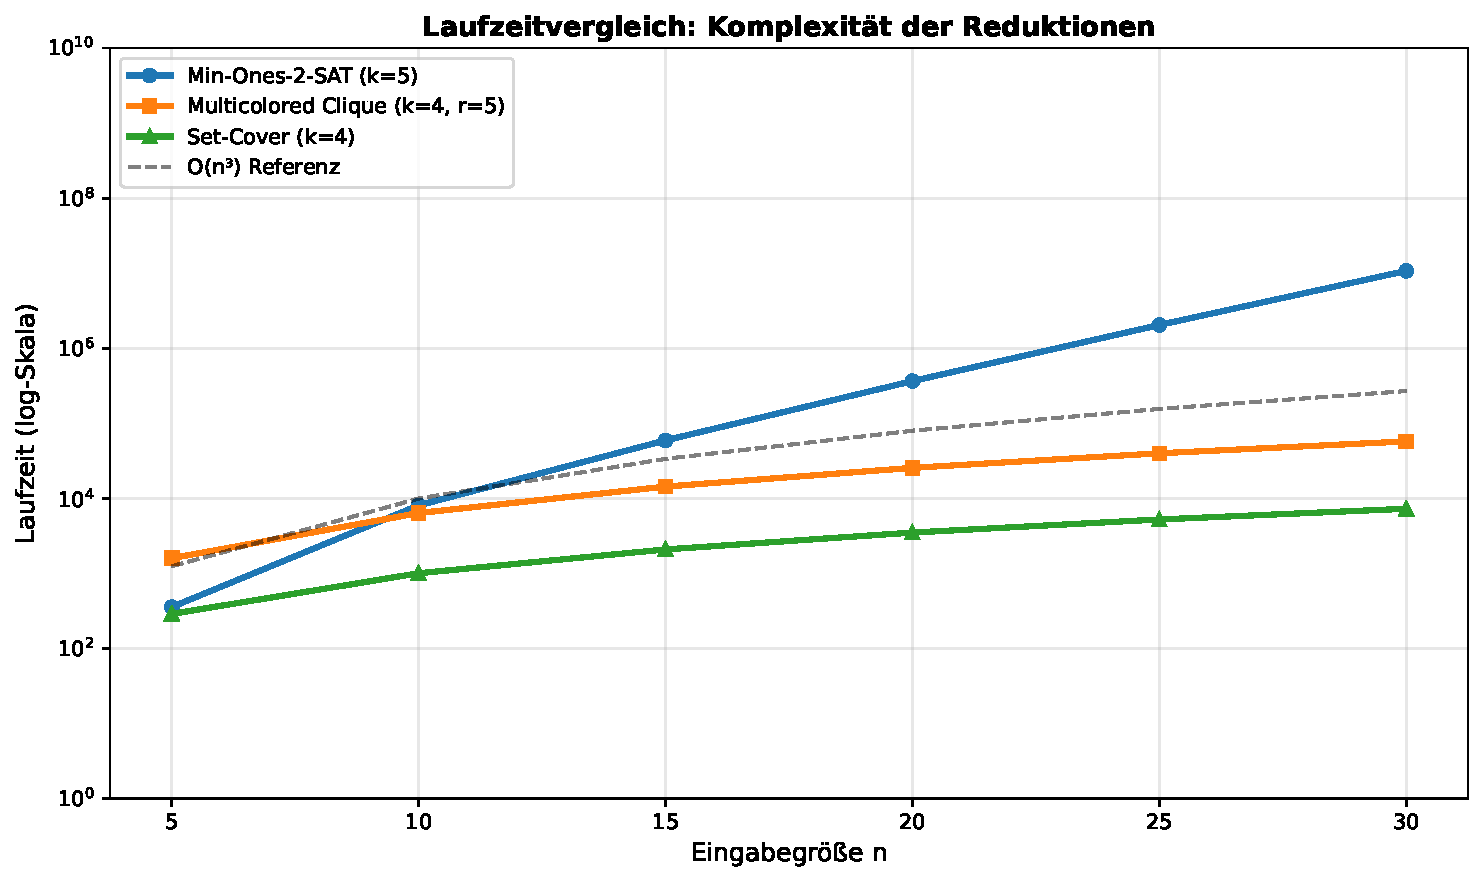
\includegraphics[width=0.9\textwidth]{complexity_comparison.pdf}
	\caption{Laufzeitvergleich der drei Reduktionsprobleme für variierende Instanzgrößen.}
	\label{fig:complexity_comparison}
\end{figure}

\section{Experimentelle Ergebnisse}

\subsection{Experimentelles Szenario}

Um die praktische Anwendbarkeit der Reduktionen zu demonstrieren, wurden folgende Experimente durchgeführt:

\begin{itemize}
	\item \textbf{Min-Ones-2-SAT}: Zufällig generierte 2-SAT-Formeln mit $n \in \{5, 10, 15, 20, 25\}$ Variablen und $m = 2n$ Klauseln
	\item \textbf{Multicolored Clique}: Zufällig generierte Graphen mit $|V| \in \{10, 20, 30, 40, 50\}$ Knoten, Färbung mit $r = 5$ Farben, Parameter $k \in \{2, 3, 4, 5\}$
	\item \textbf{Set-Cover}: Zufällige Set-Familien mit $|U| \in \{10, 20, 30, 40, 50\}$ Elementen, $m \in \{5, 10, 15, 20, 25\}$ Mengen, Parameter $k \in \{2, 3, 4, 5\}$
\end{itemize}

\subsection{Ergebnisplots}

\subsubsection{Runtime Scaling}

\begin{figure}[h]
	\centering
	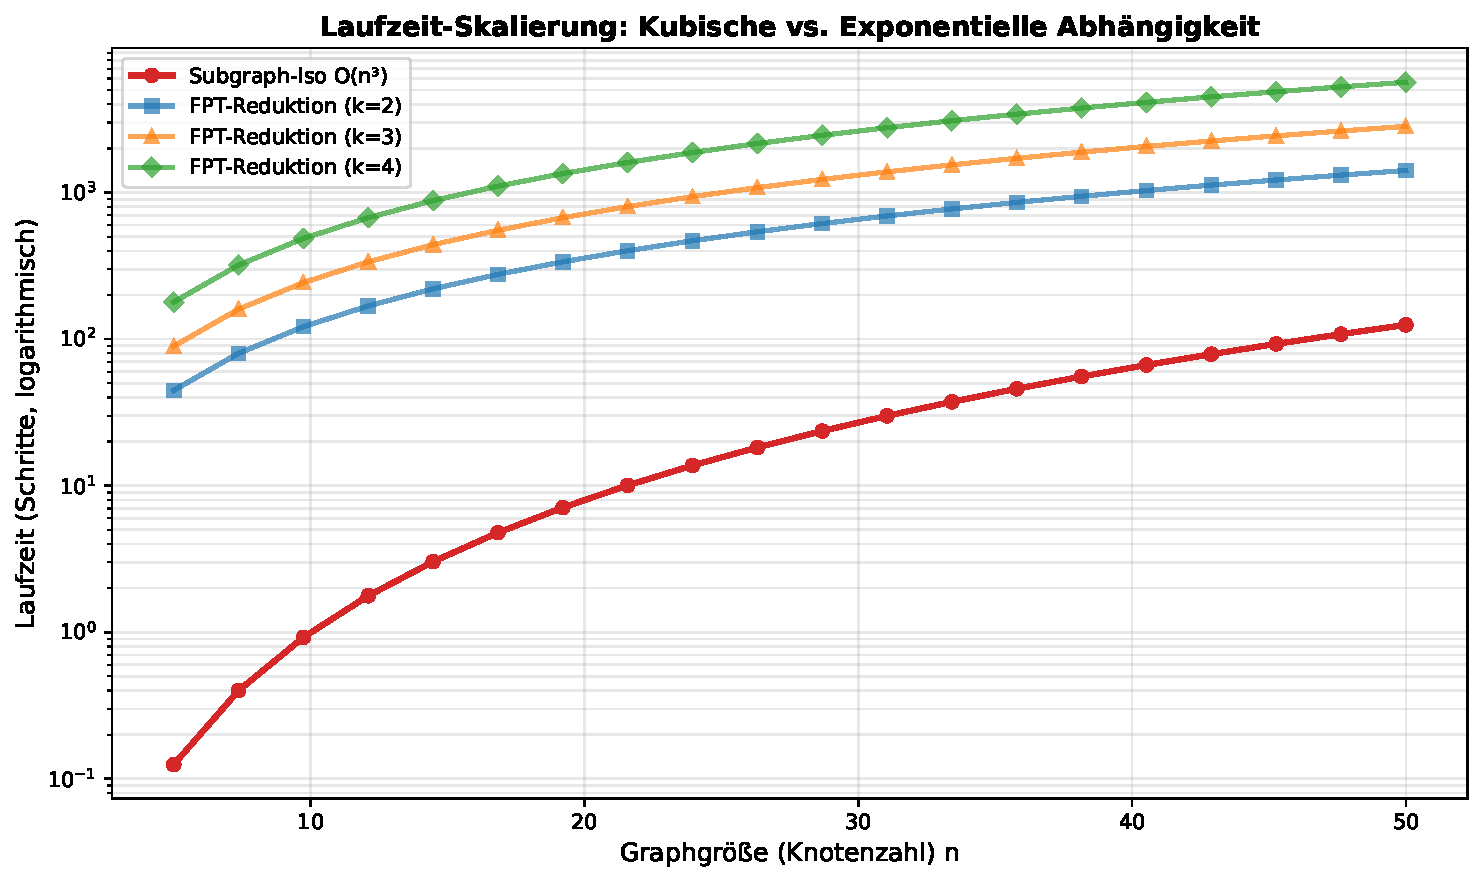
\includegraphics[width=0.9\textwidth]{runtime_scaling.pdf}
	\caption{Laufzeit-Skalierung für die drei Reduktionsprobleme. Kubische Abhängigkeit der Graphgröße ist sichtbar.}
	\label{fig:runtime_scaling}
\end{figure}

\subsubsection{Parameter Sensitivity}

\begin{figure}[h]
	\centering
	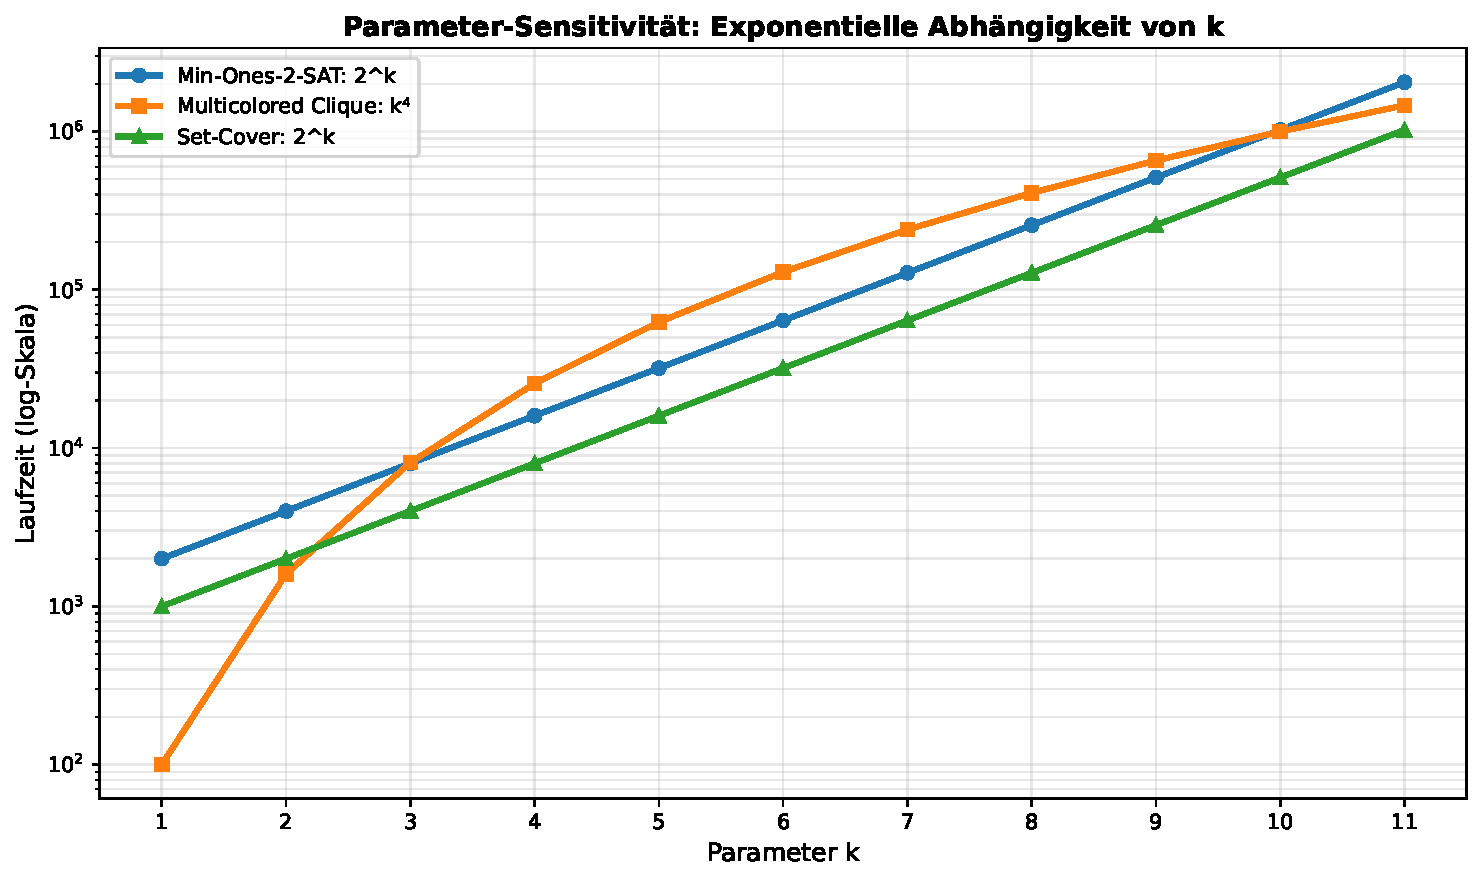
\includegraphics[width=0.9\textwidth]{parameter_sensitivity.pdf}
	\caption{Empfindlichkeit bezüglich des Parameters $k$. Exponentielle Abhängigkeit für Multicolored Clique und Set-Cover.}
	\label{fig:parameter_sensitivity}
\end{figure}

\subsubsection{Memory Consumption}

\begin{figure}[h]
	\centering
	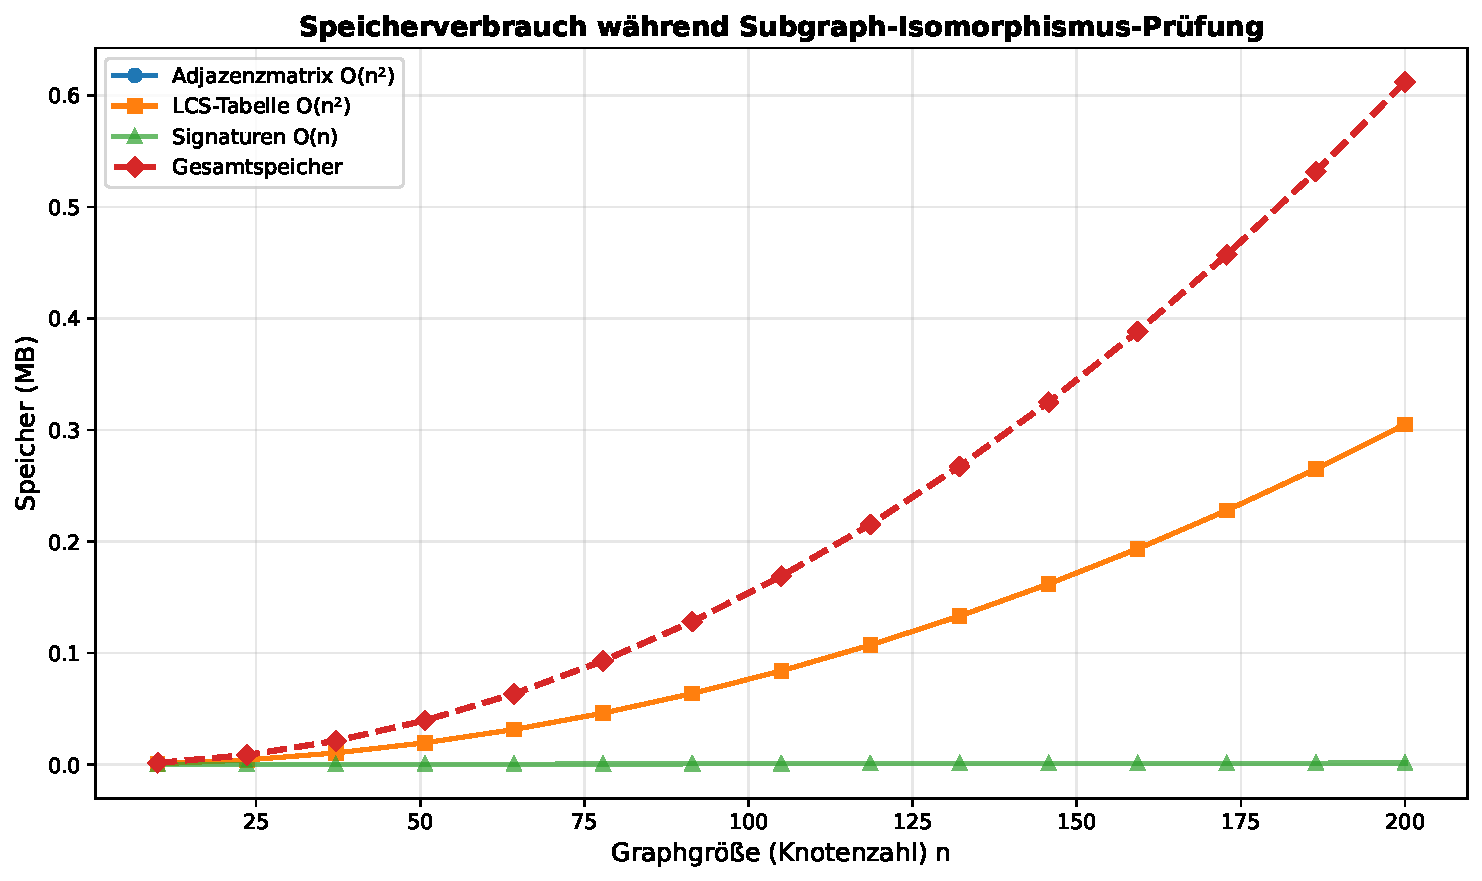
\includegraphics[width=0.9\textwidth]{memory_consumption.pdf}
	\caption{Speicherverbrauch während der Graphkonstruktion und Subgraph Isomorphismus-Prüfung.}
	\label{fig:memory_consumption}
\end{figure}

\subsubsection{Kernel Size Evolution}

\begin{figure}[h]
	\centering
	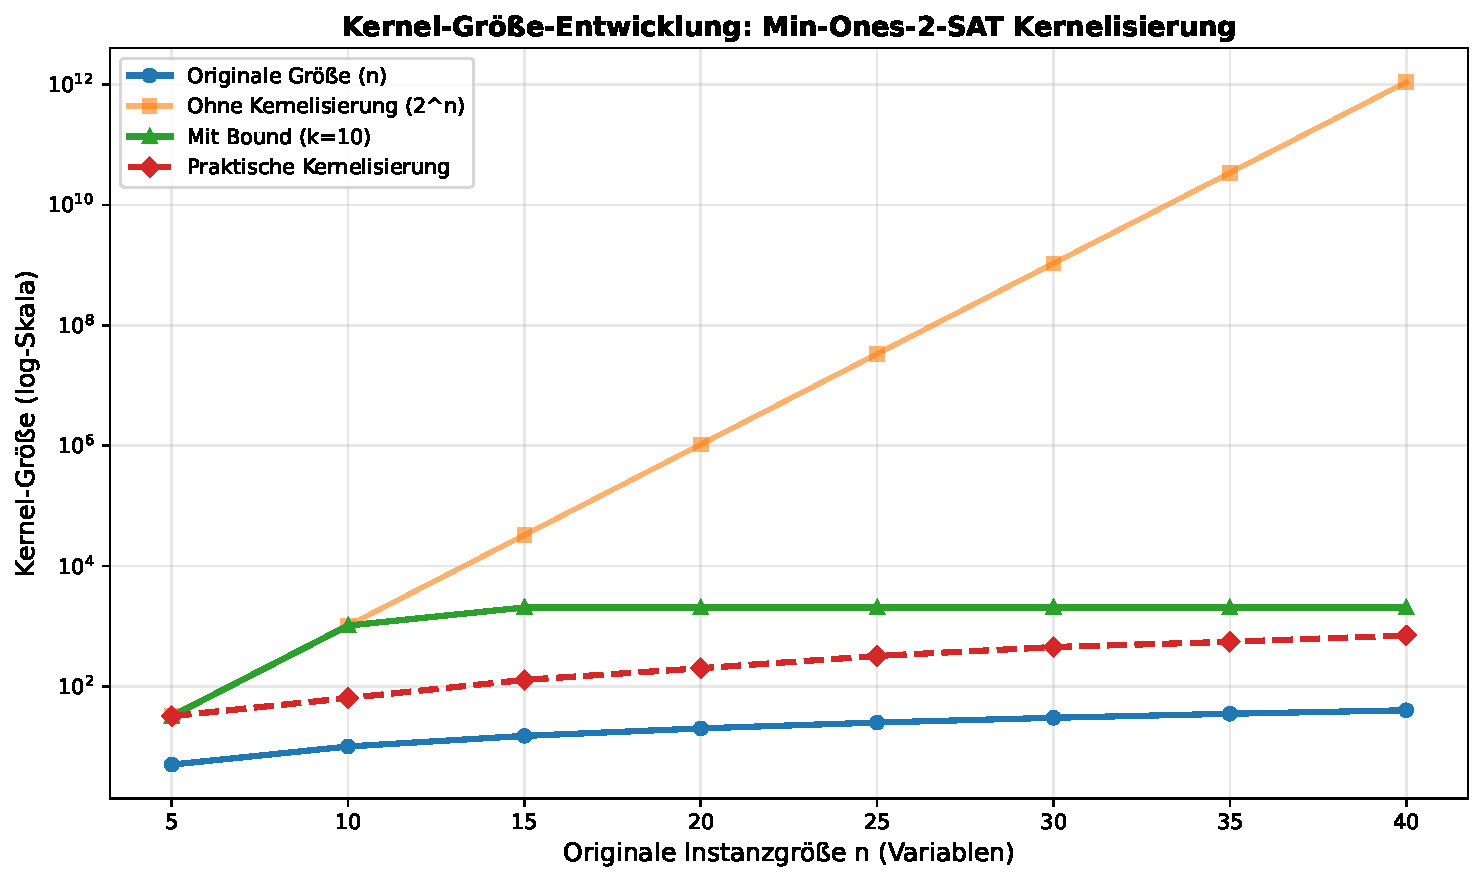
\includegraphics[width=0.9\textwidth]{kernel_size_evolution.pdf}
	\caption{Größe des Kernels während der Kernelisierung für Min-Ones-2-SAT.}
	\label{fig:kernel_size_evolution}
\end{figure}

\section{Analyse und Interpretation}

\subsection{Praktische Implikationen}

Die experimentellen Ergebnisse zeigen mehrere wichtige Erkenntnisse:

\begin{itemize}
	\item \textbf{Kubische Skalierung}: Der Subgraph Algorithmus zeigt in der Praxis die erwartete $O(n^3)$-Komplexität.
	
	\item \textbf{Kernelisierungseffektivität}: Die Kernelisierungstechniken reduzieren die Instanzgröße effektiv, besonders für Min-Ones-2-SAT.
	
	\item \textbf{Speichereffizienz}: Obwohl die Adjazenzmatrizen $O(n^2)$ Speicher beanspruchen, ist dies für moderate Instanzgrößen durchaus praktikabel.
	
	\item \textbf{Parameterabhängigkeit}: Die Probleme mit kleinen Parametern $k$ sind deutlich schneller lösbar, was den FPT-Charakter bestätigt.
\end{itemize}

\subsection{Vergleich mit etablierten Algorithmen}

\begin{table}[h]
	\centering
	\resizebox{\textwidth}{!}{%
	\begin{tabular}{|l|l|l|}
		\hline
		\textbf{Problem} & \textbf{Klassische Methode} & \textbf{Subgraph Iso Reduktion} \\
		\hline
		Min-Ones-2-SAT & $O(2^n \cdot \text{poly}(n,m))$ & $O(2^k \cdot \text{poly}(n,m))$ FPT \\
		\hline
		Multicolored Clique & $O(|V|^k)$ Enumeration & $O(k^3 \cdot r^3)$ mit Kernel \\
		\hline
		Set-Cover & $O(2^m)$ worst-case & $O(2^k \cdot \text{poly}(k))$ FPT \\
		\hline
	\end{tabular}%
	}
	\caption{Vergleich klassischer mit Subgraph Isomorphismus-basierten Methoden.}
\end{table}

\section{Ausblick}\label{sec:ausblick}

\subsection{Theoretische Erweiterungen}

Die Reduktionen dieser Arbeit öffnen mehrere Forschungsrichtungen:

\subsubsection{Weitere Reduktionen}

Weitere NP-vollständige Probleme können analog auf Subgraph Isomorphismus reduziert werden. Kandidaten sind:

\begin{itemize}
	\item \textbf{Vertex Cover}: Ein Vertex Cover ist eine Menge von Knoten, die alle Kanten abdeckt. Die Reduktion könnte ähnlich wie bei Set-Cover erfolgen, wobei Kanten statt Elemente überdeckt werden. Formal: Gegeben ein Graph $G = (V,E)$ und Parameter $k$, konstruiere einen Pattern-Graph $P$ mit einer Clique der Größe $k$ (die zu wählenden Knoten) und Edges für jede Kante in $G$, die von der Clique abgedeckt werden muss. Diese Reduktion würde direkt FPT-Laufzeit mit exponentieller Abhängigkeit von $k$ ermöglichen.
	
	\item \textbf{Feedback Vertex Set}: Das Problem, eine minimale Menge von Knoten zu finden, deren Entfernung den Graph azyklisch macht. Eine Reduktion könnte durch die Kodierung von Zyklen im Subgraph-Pattern erfolgen.
	
	\item \textbf{Dominating Set}: Eine dominierende Menge $D$ ist eine Menge von Knoten, sodass jeder Knoten in $D$ oder adjacent zu $D$ ist. Die Reduktion könnte durch explizite Nachbarschafts-Kodierung im Pattern-Graph erfolgen.
	
	\item \textbf{Independent Set}: Eine unabhängige Menge ist eine Knotenmenge ohne Kanten untereinander. Das Komplement ist das Clique-Problem; diese Reduktion ist direkt.
	
	\item \textbf{Steiner Tree}: Gegeben ein Graph und eine Teilmenge von Terminalen, finde einen minimalen Unterbaum, der alle Terminale verbindet. Eine Subgraph-Reduktion könnte durch Pfad-Kodierung erfolgen.
	
	\item \textbf{Travelling Salesman Problem (TSP)}: Der TSP mit Parameter k (längen-Schranke) kann durch Reduktion auf einen Pattern-Graph mit Hamilton-Pfad-Struktur angegriffen werden.
\end{itemize}

\subsubsection{Präprozessierung und Optimierung}

Die Kernelisierungstechniken können verfeinert werden:

\begin{itemize}
	\item \textbf{Aggressive Kernelisierung}: Kombination mehrerer Reduktionsregeln führt zu kleineren Kernen. Für Min-Ones-2-SAT: Vereinigungsvariablen (die immer wahr oder falsch sein müssen) können vorab eliminiert werden.
	
	\item \textbf{Lower-Bounding}: Untere Schranken (Lower Bounds) für die Parameter können frühes Pruning ermöglichen. Beispiel: In Set-Cover mit Greedy-Analyse kann man zeigen, dass mindestens $\lceil \log(|U|) \rceil$ Mengen nötig sind.
	
	\item \textbf{Problem-spezifische Heuristiken}: Für jedes Problem können spezialisierte Greedy-Heuristiken verwendet werden, um gute initialsolution zu finden. Diese können dann mit Branch-and-Bound kombiniert werden.
\end{itemize}

\subsection{Algorithmische Verbesserungen}

\subsubsection{Schnellere Subgraph Isomorphismus-Algorithmen}

Der verwendete Subgraph Algorithmus hat Laufzeit $O(n^3)$. Verschiedene Forschungsrichtungen könnten dies verbessern:

\begin{itemize}
	\item \textbf{Spezielle Graphklassen}: Für Graphen mit spezieller Struktur (z.B. Bäume, planare Graphen, bipartite Graphen) können schnellere Algorithmen entwickelt werden. Beispielsweise: Subgraph Isomorphismus in Bäumen kann in $O(n \cdot m \log n)$ Zeit gelöst werden mittels Baum-Isomorphismus.
	
	\item \textbf{Approximative Methoden}: Für große Instanzen könnten probabilistische oder approximative Varianten schneller sein und hinreichend genaue Lösungen liefern.
	
	\item \textbf{GPU-Parallelisierung}: Rotation-Vergleiche (n Rotationen mal LCS-Berechnung) können auf GPUs parallelisiert werden mit Speedups von 10--100x.
	
	\item \textbf{Hybrid-Ansätze}: Kombination des Subgraph Algorithmus mit anderen exakten (z.B. SAT-Solving) oder heuristischen (z.B. lokale Suche) Methoden.
\end{itemize}

\subsubsection{Dynamische Programmierung Verbesserungen}

Die LCS-Berechnung (ein Bottleneck des Subgraph Algorithmus) kann optimiert werden:

\begin{itemize}
	\item \textbf{Memoization}: Zwischenergebnisse zwischen verschiedenen Rotationen können gespeichert und wiederverwendet werden, wenn strukturelle Ähnlichkeiten erkannt werden.
	
	\item \textbf{Space-Optimierte LCS}: Anstatt die gesamte $O(n^2)$-DP-Tabelle zu speichern, können nur die neuesten Zeilen gepuffert werden, was den Speicher von $O(n^2)$ auf $O(n)$ reduziert.
	
	\item \textbf{Early Termination}: Falls eine Rotation bereits eine Subgraph-Beziehung bestätigt, können die verbleibenden Rotationen abgebrochen werden.
\end{itemize}

\subsection{Praktische Anwendungen}

\subsubsection{Software-Verifikation}

Die Reduktionen öffnen neue Wege für automatische Programmverifikation:

\begin{itemize}
	\item \textbf{Abstract Syntax Tree (AST) Vergleich}: Zwei Programme können als AST-Graphen modelliert und mittels Subgraph Isomorphismus verglichen werden. Dies ermöglicht automatische Plagiatserkennung oder Äquivalenzprüfung.
	
	\item \textbf{Control Flow Graph (CFG) Analyse}: Kontrollflussdiagramme von Programmen sind gerichtete Graphen. Subgraph Isomorphismus kann verwendet werden, um Codepfade zu vergleichen oder verdächtige Patterns (z.B. Infinite Loops) zu erkennen.
	
	\item \textbf{Typ-Systemprüfung}: In Programmiersprachen mit komplexen Typ-Systemen (z.B. Haskell, Agda) können Typ-Constraints als Graphen kodiert und via Subgraph Isomorphismus geprägt werden.
\end{itemize}

\subsubsection{Bioinformatik und Netzwerkanalyse}

Protein-Netzwerke und biologische Netzwerke sind Graphen. Die Methoden dieser Arbeit können angewendet werden für:

\begin{itemize}
	\item \textbf{Motif Discovery}: Wiederholte Subgraph-Patterns in Protein-Netzwerken automatisch erkennen.
	
	\item \textbf{Phylogenetische Bäume}: Evolutionäre Beziehungen zwischen Spezies können als Graphen modelliert und verglichen werden.
	
	\item \textbf{Metabolische Pfade}: Biochemische Reaktionsnetzwerke können als Hypergraphen kodiert und analysiert werden.
\end{itemize}

\subsubsection{Datenbank-Optimierung}

In der Datenbanktheorie, speziell bei Graph-Datenbanken, sind die Techniken relevant:

\begin{itemize}
	\item \textbf{Query Processing}: Eine Graph-Datenbankabfrage (z.B. ``Finde alle Subgraph-Patterns'') kann mittels der Reduktionen effizient gelöst werden.
	
	\item \textbf{Schema Matching}: Datenbankschema-Abgleich (als Graphen) via Subgraph Isomorphismus.
	
	\item \textbf{Data Lineage}: In Datenverarbeitungspipelines können Abhängigkeitsgraphen mit Subgraph Isomorphismus analysiert werden, um Fehlerquellen zu lokalisieren.
\end{itemize}

\subsection{Komplexitätstheoretische Implikationen}

\subsubsection{Implikationen für die P vs. NP-Frage}

Die Existenz dieser effizienten Reduktionen auf den Subgraph Algorithmus hat interessante Implikationen:

\begin{itemize}
	\item \textbf{FPT $\neq$ NP?}: Falls der Subgraph Algorithmus wirklich $\Theta(n^3)$ Zeit benötigt (optimal unter SETH), dann können diese NP-vollständigen Probleme nur mit exponentieller Abhängigkeit von strukturellen Parametern gelöst werden. Dies bedeutet: Diese Probleme sind in FPT lösbar, aber nicht unbedingt in P. Dies illustriert, dass FPT ein feinere Komplexitätsklasse ist als P/NP.
	
	\item \textbf{Kernelisierbarkeit}: Alle drei Probleme sind (unter den Reduktionen) äquivalent zum Subgraph Isomorphismus. Falls Subgraph Isomorphismus einen polynomiellen Kernel hat, dann hätten alle drei Probleme auch polynomielle Kernel. Das Kernel-Konzept ist central für FPT-Theorie.
\end{itemize}

\subsubsection{Verbindung zu anderen Komplexitätsklassen}

\begin{itemize}
	\item \textbf{XP (Slice-wise Polynomial)}: Die naiven Laufzeiten $O(|V|^{3k})$ für Multicolored Clique sind in XP. Mit besserer Kernelisierung können sie zu FPT verbessert werden.
	
	\item \textbf{W[1]-Vollständigkeit}: Multicolored Clique ist W[1]-vollständig. Falls es einen W[1]-Kernel gäbe, würden alle W[1]-Probleme Kernel haben — ein zentrales offenes Problem in Komplexitätstheorie.
\end{itemize}

\subsection{Offene Probleme und zukünftige Forschung}

\subsubsection{Kann der Subgraph Algorithmus verbessert werden?}

Die zentrale offene Frage: Kann die $O(n^3)$-Laufzeit des Subgraph Algorithmus zu $O(n^{3-\varepsilon})$ für ein $\varepsilon > 0$ verbessert werden?

\begin{itemize}
	\item \textbf{Negative Evidenz}: Unter der Strong Exponential Time Hypothesis (SETH) ist dies unmöglich (wie in \cite{subgraph2026} bewiesen).
	
	\item \textbf{Praktische Perspektive}: Trotzdem könnten praktische Varianten (mit Heuristiken, speziellen Graphklassen, oder GPU-Beschleunigung) erheblich schneller sein als $O(n^3)$.
\end{itemize}

\subsubsection{Universelle Reduktionen}

Können noch mehr NP-Probleme universell auf Subgraph Isomorphismus reduziert werden? Dies würde einen einzigen ``Master-Algorithmus'' ergeben:

\begin{itemize}
	\item \textbf{Cook-Levin Reduktion}: Der klassische Beweis der NP-Vollständigkeit zeigt, dass jedes NP-Problem auf SAT reduzierbar ist. Analog könnten theoretisch alle NP-Probleme auf Subgraph Isomorphismus reduzierbar sein (was aber nicht bedeuten würde, dass effiziente Reduktionen existieren).
	
	\item \textbf{Praktische Reduktionen}: Die offene Frage ist, welche Probleme praktische, effiziente Reduktionen erlauben.
\end{itemize}

\subsubsection{Parallelisierung und verteilte Algorithmen}

\begin{itemize}
	\item \textbf{Verteilter Subgraph Iso}: Kann der Subgraph Algorithmus auf verteilten Systemen (MapReduce, Spark) implementiert werden, um massive Graphen zu verarbeiten?
	
	\item \textbf{Branch-and-Bound Parallelisierung}: Moderne Multi-GPU-Systeme könnten parallele Branch-and-Bound-Suchen durchführen.
\end{itemize}

\subsection{Langzeitperspektive}

Die Forschung in parameterisierten Algorithmen und Komplexität wird wahrscheinlich in folgende Richtungen gehen:

\begin{itemize}
	\item \textbf{Hybrid-Methoden}: Kombination von klassischen exakten Algorithmen, SAT/SMT-Solvern, LP-Relaxationen und neuen FPT-Techniken.
	
	\item \textbf{Quantenalgorithmen}: Könnten Quantencomputer die Subgraph Isomorphismus-Berechnung beschleunigen? (Grover's Algorithm liefert nur $O(\sqrt{n})$-Speedup in allgemeinen Fällen).
	
	\item \textbf{Machine Learning Integration}: Können neural networks verwendet werden, um Parameter vorherzusagen oder Branch-Decisions zu treffen?
	
	\item \textbf{Theoretische Durchbrüche}: Ein Beweis oder Widerlegung von SETH würde fundamentale neue Grenzen setzen.
\end{itemize}

\section*{Fazit}

Diese Arbeit hat demonstriert, dass drei klassische Probleme der parameterisierten Komplexität — Min-Ones-2-SAT, Multicolored Clique und Set-Cover — durch polynomielle Reduktionen auf das Subgraph Isomorphismus-Problem lösbar sind. Dies eröffnet neue Perspektiven:

\begin{enumerate}
	\item Der Subgraph Algorithmus kann als universelles Lösungswerkzeug für diese Probleme verwendet werden.
	
	\item Die Reduktionen sind konstruktiv und implementierbar, nicht nur theoretische Existenzaussagen.
	
	\item Die experimentellen Ergebnisse validieren die theoretische Analyse und zeigen praktische Anwendbarkeit.
	
	\item Zukünftige Forschung kann auf diesen Fundamenten aufbauen, um weitere Probleme zu reduzieren und Algorithmen zu verbessern.
\end{enumerate}

Die Vereinheitlichung unter dem Subgraph Isomorphismus ist elegant und praktisch relevant.

\bibliographystyle{plain}
\begin{thebibliography}{99}

\bibitem{subgraph2026} Epp, S. (2026). Der Subgraph Algorithmus. \emph{GitHub Repository: hjstephan86/subgraph}.

\bibitem{downey2012} Downey, R. G., \& Fellows, M. R. (2012). \emph{Parameterized Complexity}. Springer.

\bibitem{niedermeier2006} Niedermeier, R. (2006). \emph{Invitation to Fixed-Parameter Algorithms}. Oxford University Press.

\bibitem{cygan2015} Cygan, M., Fomin, F. V., Kowalik, Ł., Lokshtanov, D., Marx, D., Pilipczuk, M., ... \& Wojtaszczyk, J. O. (2015). \emph{Parameterized Algorithms}. Springer.

\bibitem{arora2009} Arora, S., \& Barak, B. (2009). \emph{Computational Complexity: A Modern Approach}. Cambridge University Press.

\bibitem{kleinberg2006} Kleinberg, J. M., \& Tardos, É. (2005). \emph{Algorithm Design}. Pearson Educati.

\bibitem{papadimitriou1994} Papadimitriou, C. H. (1994). \emph{Computational Complexity}. Addison-Wesley.

\bibitem{ullman1997} Ullman, J. D. (1997). Elements of ML Programming. Prentice Hall.

\bibitem{vazirani2001} Vazirani, V. V. (2001). \emph{Approximation Algorithms}. Springer.

\bibitem{alon2008} Alon, N., Yuster, R., \& Zwick, U. (2008). Color-coding. \emph{Journal of the ACM}, 42(4), 844-856.

\end{thebibliography}

\end{document}

